 % -*- mode: LaTeX -*-
 % ... preamble ...
\documentclass[times,12pt,titlepage]{mstthesis}
\doublespacing
\usepackage{threeparttable}
\usepackage[final]{graphicx}
\usepackage{psfrag}
\usepackage[noprefix]{nomencl}
\makenomenclature
\renewcommand{\nomgroup}[1]{
   \ifthenelse{\equal{#1}{A}}{\medskip \item \textbf{Roman}}{}%
   \ifthenelse{\equal{#1}{G}}{\medskip \item \textbf{Greek}}{}%
   \ifthenelse{\equal{#1}{S}}{\medskip \item \textbf{Subscripts}}{}%
}
\usepackage[nopar]{lipsum} % ... provides dummy text ...

 % ... end preamble ...

\begin{document}

 % ... specify: ms or phd ...

\begin{ThesisTitlePage}{ms}

 % ... title page info ...

\author{\MakeUppercase{I. M. Author}}

\thesistitle{\MakeUppercase{The Title of My Work}}

\department{Mechanical Engineering}

 % ... thesis committee ...

\ThesisAdviser{Galileo}

 % If you have a co-advisor, enter the name in the
 % curly braces below and uncomment.
 % Otherwise, leave commented out.
 %\cothadviser{} % If you have 2 thesis advisers

\memberone{Newton}
\membertwo{Copernicus}
\memberthree{Laplace}
\memberfour{Fourier}
\memberfive{Prandtl}

 % ... Graduation date - NOT your submission date ...
\graddate{1685}

\end{ThesisTitlePage}
 % ... copyright page - true|false ...

\copyrightyear{1684}
\ThesisCopyrightPage{true}

 % ... front matter - thesis abstract ...

\begin{ThesisAbstract}
\lipsum[1]
\end{ThesisAbstract}

 % ... front matter - thesis acknowledgements ...

\begin{ThesisAcknowledgment}
\lipsum[2]
\end{ThesisAcknowledgment}
\begin{ThesisFrontMatter}
\tableofcontents
\listoffigures
\listoftables
\listofsymbols
\end{ThesisFrontMatter}

\begin{ThesisBody}

 % ... introduction chapter ...
\ThesisBodyChapter{Introduction}%%
%% This is file `chapmin.tex',
%% generated with the docstrip utility.
%%
%% The original source files were:
%%
%% ths.dtx  (with options: `chapmin')
%% 
%% IMPORTANT NOTICE:
%% 
%% For the copyright see the source file.
%% 
%% Any modified versions of this file must be renamed
%% with new filenames distinct from chapmin.tex.
%% 
%% For distribution of the original source see the terms
%% for copying and modification in the file ths.dtx.
%% 
%% This generated file may be distributed as long as the
%% original source files, as listed above, are part of the
%% same distribution. (The sources need not necessarily be
%% in the same archive or directory.)


 %% ... sample chapter ...

\lipsum[5]

\section{Introduction}
\lipsum[6-8]

\endinput
%%
%% End of file `chapmin.tex'.


 % ... conclusions chapter ...
\ThesisBodyChapter{Conclusions}%%
%% This is file `chapall.tex',
%% generated with the docstrip utility.
%%
%% The original source files were:
%%
%% ths.dtx  (with options: `chapmin,addfig,addtbl,addbib,addglo')
%% 
%% IMPORTANT NOTICE:
%% 
%% For the copyright see the source file.
%% 
%% Any modified versions of this file must be renamed
%% with new filenames distinct from chapall.tex.
%% 
%% For distribution of the original source see the terms
%% for copying and modification in the file ths.dtx.
%% 
%% This generated file may be distributed as long as the
%% original source files, as listed above, are part of the
%% same distribution. (The sources need not necessarily be
%% in the same archive or directory.)


 %% ... sample chapter ...

\lipsum[5]

\section{Introduction}
\lipsum[6-8]

\section{Section with Figures and Heading Which is Really Long So
That It Produces a Two-Line Toc Entry}
\lipsum[9]

\subsection{Simple Figure with Label}

Add a simple figure, Figure~\ref{fig:fig00}, to illustrate
an entry in the list of figures. %
\begin{figure}[tb]
  \begin{center}
   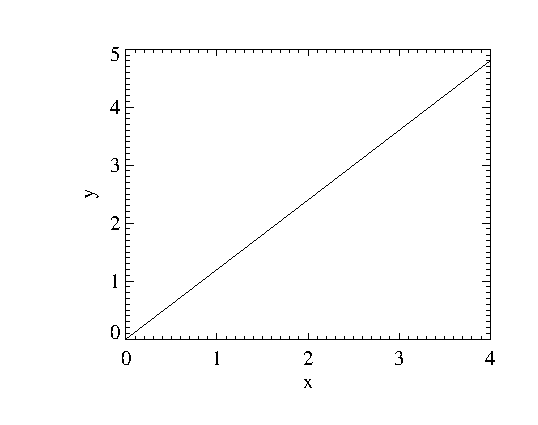
\includegraphics[width=3.75in]{simple.eps}
  \end{center}
  \caption{The caption of the figure.}
\label{fig:fig00}
\end{figure}%
\lipsum[5]

\subsection{Figure with psfrag Replacement}

\lipsum[8].  Figure~\ref{fig:fig01} illustrates the use
of the psfrag package to place \LaTeX\ math in a graphic.%
\begin{figure}[tb]
  \psfrag{x}{$x$}
  \psfrag{y}{$y$}
  \begin{center}
   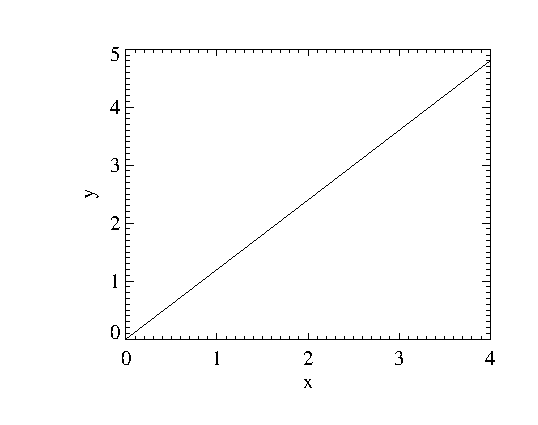
\includegraphics[width=3.75in]{simple.eps}
  \end{center}
  \caption[A figure caption which is extra long.]{A figure caption
    which is extra long. This long caption not only demonstratees that
    the required spacing in the list of figures is correct, but also
    the general practice of making the list of figures (or tables)
    entry the first sentence of the caption.}
\label{fig:fig01}
\end{figure}
\lipsum[1]. The filler content is followed by a second figure,
Figure~\ref{fig:fig02}.  %
\begin{figure}[tb]
  \psfrag{x}{$\hat{x}/L$}
  \psfrag{y}{$y$}
  \begin{center}
   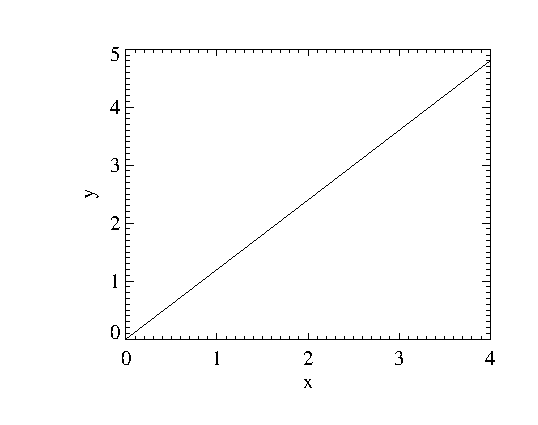
\includegraphics[width=3.75in]{simple.eps}
  \end{center}
  \caption{The figure caption made extra long so that the
    required spacing in the list of figures is evident.}
\label{fig:fig02}
\end{figure}
\lipsum[9]
\section{Section with Sample Tables}

\subsection{Simple Table}

Finally the tables, Table~\ref{tbl:tbl01} illustrates the syntax of a
basic table. %
\begin{table}[tb]
  \caption{The capitalization of the table should match that of figures.}
  \label{tbl:tbl01}
  \begin{center}
  \begin{tabular}{c l l}
  \hline
  Example & Time & Cost \\
  \hline
  1 & 12.5 & \$1,000 \\
  2 & 24 & \$2,000 \\
  \hline
  \end{tabular}
  \end{center}
\end{table}

\subsection{Three-Part Table}

Table~\ref{tbl:tbl02}, which illustrates the syntax of a three-part
table which includes table notes in addition to a caption and table
body.
\begin{table}[tb]
\begin{threeparttable}
  \caption{The caption of the three-part table.}
  \label{tbl:tbl02}
  \begin{center}
\begin{tabular*}{\textwidth}{c l l} % or {tabular}
  \hline
  Example & Time\tnote{1} & Cost \\
  \hline
  1 & 12.5 & \$1,000 \\
  2 & 24 & \$2,000 \\
  \hline
\end{tabular*}
\begin{tablenotes}
  \item [1] The first note.
\end{tablenotes}
  \end{center}
\end{threeparttable}
\end{table}
\lipsum[11-12]


\section{Section with \texttt{natbib} Citations}

This had been discussed previously by \citep{bullwinkle:1990} and
\citet{bullwinkle:1991}. \lipsum[10-11]


\section{Section with \texttt{nomencl} Entries}

 This is my simple equation to illustrate the use of the nomencl
 package for automatic generation of a list of symbols.
\begin{equation}
\delta_i = \sqrt{t/\mathrm{Pe}}
\end{equation}
where $\delta$ is the layer
thickness %
\nomenclature[at]{$t$}{time}%
\nomenclature[gd]{$\delta$}{layer thickness}%
\nomenclature[si]{$i$}{inlet}%
as defined previously. \lipsum[13]
\endinput
%%
%% End of file `chapall.tex'.


\end{ThesisBody}
 % ... appendix - specify number of appendix chapters ...

\begin{ThesisAppendix}{two}
\ThesisAppendixChapter{One}%%
%% This is file `chapbib.tex',
%% generated with the docstrip utility.
%%
%% The original source files were:
%%
%% ths.dtx  (with options: `chapmin,addbib')
%% 
%% IMPORTANT NOTICE:
%% 
%% For the copyright see the source file.
%% 
%% Any modified versions of this file must be renamed
%% with new filenames distinct from chapbib.tex.
%% 
%% For distribution of the original source see the terms
%% for copying and modification in the file ths.dtx.
%% 
%% This generated file may be distributed as long as the
%% original source files, as listed above, are part of the
%% same distribution. (The sources need not necessarily be
%% in the same archive or directory.)


 %% ... sample chapter ...

\lipsum[5]

\section{Introduction}
\lipsum[6-8]


\section{Section with \texttt{natbib} Citations}

This had been discussed previously by \citep{bullwinkle:1990} and
\citet{bullwinkle:1991}. \lipsum[10-11]

\endinput
%%
%% End of file `chapbib.tex'.

\ThesisAppendixChapter{Two}%%
%% This is file `chapbib.tex',
%% generated with the docstrip utility.
%%
%% The original source files were:
%%
%% ths.dtx  (with options: `chapmin,addbib')
%% 
%% IMPORTANT NOTICE:
%% 
%% For the copyright see the source file.
%% 
%% Any modified versions of this file must be renamed
%% with new filenames distinct from chapbib.tex.
%% 
%% For distribution of the original source see the terms
%% for copying and modification in the file ths.dtx.
%% 
%% This generated file may be distributed as long as the
%% original source files, as listed above, are part of the
%% same distribution. (The sources need not necessarily be
%% in the same archive or directory.)


 %% ... sample chapter ...

\lipsum[5]

\section{Introduction}
\lipsum[6-8]


\section{Section with \texttt{natbib} Citations}

This had been discussed previously by \citep{bullwinkle:1990} and
\citet{bullwinkle:1991}. \lipsum[10-11]

\endinput
%%
%% End of file `chapbib.tex'.

\end{ThesisAppendix}

 % ... references - comma separated list of bib files ...

\newpage\bibliographystyle{plainnat}
\bibliography{add.bib}

 % ... vita ...

\begin{Vita}
\lipsum[3]
\end{Vita}

\end{document}
